\chapter{Analyse}

\section{Manipulationssichere Datenstrukturen}
Wie im Kapitel Vulnerabilität beschrieben ist es schwierig, Manipulation von Daten durch autorisierte Benutzer zu verhindern. Jedoch ist es möglich Manipulationen zu entdecken. Damit diese Erkennung funktioniert, muss die Datenstruktur einige Mechanismen unterstützen: \\
Das Hinzufügen eines Eintrags $X\textsubscript{i}$ in die Datenstruktur erzeugt eine Verifikation $C\textsubscript{i}$.\\
$Add(X) {\rightarrow} C\textsubscript{i}$.\\
Aus dieser Verifikation kann ein inkrementeller Beweis angefertigt werden, der die direkte Nachbarschaft zweiter Elemente belegt \\
$VerInc(X\textsubscript{i}, C\textsubscript{i-1}) {\rightarrow} C\textsubscript{i}$. \\
Wenn es zwei Elemente $C\textsubscript{i}$ und $C\textsubscript{j}$ aus der Datenstruktur gibt, dann gibt es eine eindeutige Reihenfolge von $i > j$ oder $i < j$. In beiden Fällen kann ein transitiver Beweis erstellt werden, der belegt, dass es eine konsistente Verbindung zwischen den beiden Elementen gibt und somit die Konsistenz des Logs zwischen $i$ und $j$ belegt $VerMember(C\textsubscript{i}, C\textsubscript{j}) {\rightarrow} ({\top},{\perp})$. \\
Mit diesen Grundregeln kann bewiesen werden, dass ein Element zur Datenstruktur gehört und es kann ein beliebig großer Ausschnitt des Logs verifiziert werden. \cite{8280477}\\
\\
\subsection{Analyse Hashchains}
Wie in Kapitel Grundlagen beschrieben sind Hashchains eine in sich abgesicherte Datenstruktur.Durch ihre rekursive Erstellung ist diese gut für die Audit-Log-Führung geeignet. Elemente in einer Hashchain haben immer eine feste Reihenfolge. Die Konsistenz zwischen Elementen kann überprüft werden, da die Hashchain von jedem Punkt aus mit dem dortigen Hashwert und den darauffolgenden Elementen neu berechnet werden kann. Wenn nun das Ergebnis des neuberechneten Hashwertes vom erwarteten Hashwert abweicht, ist bewiesen, dass die Daten nicht in ihrem Ursprungszustand vorliegen. \\
Hashchains haben für das Einfügen von Elementen eine konstante Komplexität. Die benötigte Zeit beim Überprüfen von Elementen ist linear.\cite[S.351ff]{40322788} \\
\\
\subsection{Analyse Merkle tree}
Merkle trees erfüllen die Anforderungen ebenfalls. Durch ihre Baumstruktur erhalten sie den Zugriff auf alle Blätter in logarithmischer Zeit. Bei der Verwendung von Merkle trees gibt es aber einige Besonderheiten zu beachten.\\
Die größte Nachteil ist, dass sich beim Hinzufügen von Einträgen (Blättern) Einträge in der Datenstruktur ändern anstatt lediglich die neuen Daten anzuhängen. Es ändern sich je nach Baumgröße und momentanen Zustand interne Knoten. Dies erfordert eine erneute Berechnung aller Knoten ab der Änderung bis zur Wurzel, um die Integrität des Baumes wieder herzustellen. Dieses Verhalten hat zwei Probleme zur Folge: Wenn nur ein einzelner Wert (die Wurzel), wie bei statischen Daten, als Verifikation gespeichert wird, dann verliert diese bei jeder Änderung ihre Gültigkeit. Solange der Baum klein ist, ist der Aufwand zum Einfügen eines Knotens noch gering, jedoch steigt der Aufwand je größer der Baum wird. Um den Aufwand zum Einfügen der Knoten zu verringern kann man den Baum so anlegen, dass alle Blätter des Baumes dieselbe Tiefe besitzen. Wenn der Baum voll ist, wird der Baum nicht neu ausbalanciert, sondern es wird über der Wurzel ein neuer Knoten eingesetzt. Der daraus resultierende Baum hat damit die Kapazität für doppelt so viele Blätter. Dieses Vorgehen hat den Vorteil, dass möglichst viele Knoten im Baum so früh wie möglich einen finalen Wert und feste Position beziehen. So können Beweise abgespeichert werden, die maximal einen Knoten pro Ebene des Baumes beinhalten. Ein Knoten des Baumes, der sich nicht mehr ändert, beweist die Konsistenz aller Knoten und Blätter unter sich. \\
Ein weiterer Nachteil ist, dass zum Erweitern der Bäume nicht nur ein simpler Top-Hash nötig ist, sondern eine beliebig große Menge von Daten kann Einfluss auf neu eingefügte Elemente haben. Dies kann bei beliebig großen Bäumen und begrenztem Arbeitsspeicher problematisch werden. Die Menge an Informationen die aus einem Baum minimal benötigt wird kann durch einen Algorithmus zur Findung von minimalen Verifikation eines Baumzustands erlangt werden.\cite{8280477} \cite{8280476}\\ 
\clearpage
Der Einfügeprozess anhand eines Beispiels: \\
Im Folgenden betrachten wir das beispielhafte Erweitern eines Merkle trees von der initialen Größe von sechs Knoten um jeweils einen Knoten in vier Schritten. Dabei erhalten wir einen Einblick in die Best- und Worst-Case Szenarien. Für die Legende der Abblidungen siehe Tabelle \ref{tab:TreeProofTable1}.

\begin{table}[!htb]
\caption{Legende: Einfügeoperation}
\label{tab:TreeProofTable1}
\begin{tabular}{|l|l|}
\hline
\textbf{Knoten} & \textbf{Beschreibung}
\\ \hline
Grün & \begin{tabular}[x]{@{}l@{}}Kleinste Menge an Knoten für einen Beweis für den neu eingefügten\\
Knoten. Diese Knoten sind bereits stabil und werden sich durch weitere \\
Einfüge-Operationen nicht mehr ändern.\end{tabular}
\\ \hline
Orange & \begin{tabular}[x]{@{}l@{}}Diese Knoten sind instabil und werden sich beim Erweitern des Baumes\\
noch ändern.\end{tabular}
\\ \hline
Blau & \begin{tabular}[x]{@{}l@{}}Stabile Knoten, die nicht zum Beweis gehören. Deren Hashwert wurde\\
bereits für die Erstellung der aktuell grünen Knoten verwendet\\
und diese konnten somit vernachlässigt werden.\end{tabular}
\\ \hline
Weiß & \begin{tabular}[x]{@{}l@{}}Weiße Knoten sind Platzhalter für später einzufügende Knoten. Diese\\
Knoten entstehen nur als rechter Knoten zu einem einzelnen Knoten\\
ohne Partner, damit der Baum bis zur Wurzel berechnet werden kann.\\
Der Hashwert dieser Knoten entspricht dem seines Nachbarns.\end{tabular}
\\ \hline
\end{tabular}
\end{table}

\begin{figure}[!htb]
	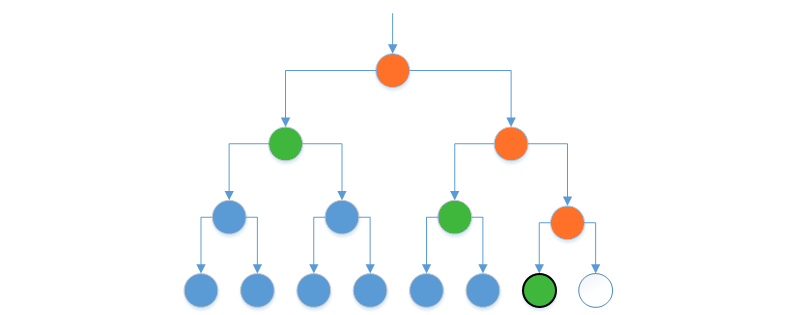
\includegraphics[width=1\textwidth]{content/pictures/TreeProof1}
	\caption{Schritt 1: einfügen Knoten 7}
	\label{fig:TreeProof1}
\end{figure}

In Schritt eins (siehe Abbildung \ref{fig:TreeProof1}) wird der siebte Knoten eingefügt. Als Beweis werden das Blatt selbst, und ein Knoten aus jeder Ebene außer der Wurzel gespeichert. Dies ist der Worst-Case da dies die maximal benötigte Anzahl an Knoten für diese Baumgröße ist. Der weiße Platzhalter-Knoten wird benötigt um den Baum bis zur Wurzel berechnen zu können und stellt darüber hinaus sicher, dass in allen höheren Ebenen Änderungen auftreten sobald der Platzhalter duch einen normalen Knoten ersetzt wird. Somit ist auch die Stabilität des Baums der Worst-Case, da in jeder Ebene außer den Blättern ein instabiler Knoten existiert.\\
\begin{figure}[!htb]
	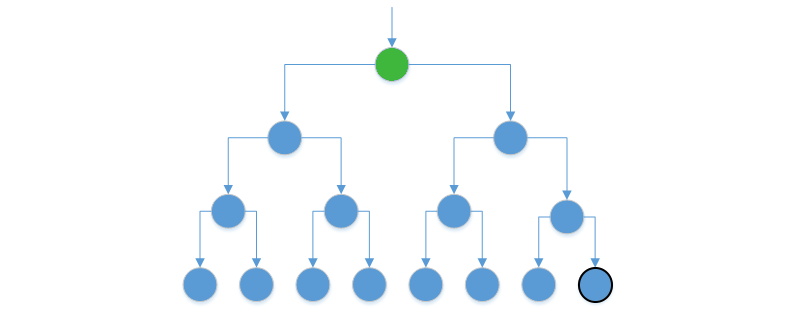
\includegraphics[width=1\textwidth]{content/pictures/TreeProof2}
	\caption{Schritt 2: einfügen Knoten 8}
	\label{fig:TreeProof2}
\end{figure}
\\
Im Gegensatz dazu ist Schritt zwei (siehe Abbildung \ref{fig:TreeProof2}) ein Best-Case. Der Baum ist voll und daher ist nun die Wurzel stabil und kann als Beweis für alle Unterknoten verwendet werden. Außerdem ist der Baum komplett stabil und es existieren keine instabilen Knoten.\\
\begin{figure}[!htb]
	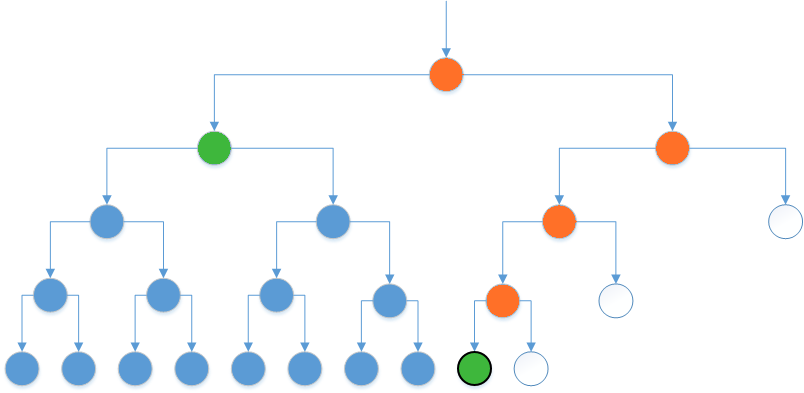
\includegraphics[width=1\textwidth]{content/pictures/TreeProof3}
	\caption{Schritt 3: einfügen Knoten 9}
	\label{fig:TreeProof3}
\end{figure}
\\
In Schritt drei (siehe Abbildung \ref{fig:TreeProof3}) muss der Baum, um den neunten Knoten einzufügen, erweitert werden. Da der Baum nicht neu balanciert wird, bleibt der alte Unterbaum stabil und es werden für jede Baumebene außer der Wurzel, temporäre Knoten verwendet, um den nächsten Knoten einzufügen. Der Beweis für diese Baumkonfiguration besetht aus der letzten Probe und dem neuen Knoten. Die Stabilität ist erneut ein Worst-Case, da es maximal viele instabile Knoten gibt.\\
\begin{figure}[!htb]
	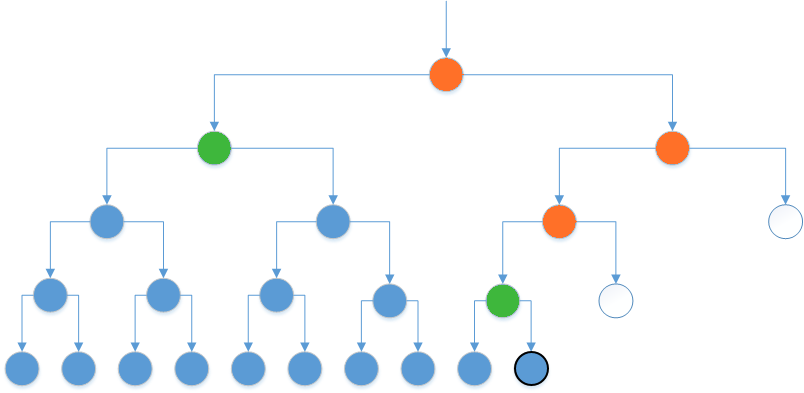
\includegraphics[width=1\textwidth]{content/pictures/TreeProof4}
	\caption{Schritt 4: einfügen Knoten 10}
	\label{fig:TreeProof4}
\end{figure}
\\
Zuletzt wird in Schritt vier (siehe Abbildung \ref{fig:TreeProof4}) der zehnte Knoten eingefügt, welcher bereits einen stabilen Knoten im neuen Unterbaum erzeugt. Die Menge an temporären und instabilen Knoten wurde jeweils um eins reduziert.\\

Zum Beweisen der Nachbarschaft zweier Knoten kann analog zu einer normalen Hashchain aus dem Beweis der Konsistenz des Vorgängerknoten und dem aktuellen Knoten der Beweis des Knotens rekonstruiert werden. Ist der Knoten unverändert, wird dies durch ein identisches Ergebnis bestätigt.\\

Um Knoten acht zu überprüfen (siehe Abbildung \ref{fig:TreeProof5} und Tabelle \ref{tab:TreeProofTable2}) wird der Beweis von Knoten sieben (in Gelb dargestellt) und der zu überprüfende Knoten selbst (in lila) gebraucht. Wenn nun der grüne Beweisknoten durch erneuerte Berechnung auf Basis des Beweises seines Vorgängers errechnet werden kann, ist die Konsistenz bewiesen.
\clearpage 
\begin{table}[!htb]
\caption{Legende: Beweiskonstruktion}
\label{tab:TreeProofTable2}
\begin{tabular}{|l|l|}
\hline
\textbf{Knoten} & \textbf{Beschreibung}
\\ \hline
Lila & \begin{tabular}[x]{@{}l@{}}Zu prüfender Knoten\end{tabular}
\\ \hline
Gelb & \begin{tabular}[x]{@{}l@{}}Beweis für den Vorgängerknoten des zu prüfenden Knotens.\end{tabular}
\\ \hline
Grün & \begin{tabular}[x]{@{}l@{}}Beweis des zu prüfenden Knotens.\end{tabular}
\\ \hline
Orange & \begin{tabular}[x]{@{}l@{}}Knoten, die für die Rekonstruktion des grünen Beweises erneut\\
berechnet werden müssen.\end{tabular}
\\ \hline
Blau & \begin{tabular}[x]{@{}l@{}}Für diesen Fall irrelevante Knoten.\end{tabular}
\\ \hline
Weiß & \begin{tabular}[x]{@{}l@{}}Platzhalter Knoten für diesen Fall irrelevant.\end{tabular}
\\ \hline
\end{tabular}
\end{table}

\begin{figure}[!htb]
	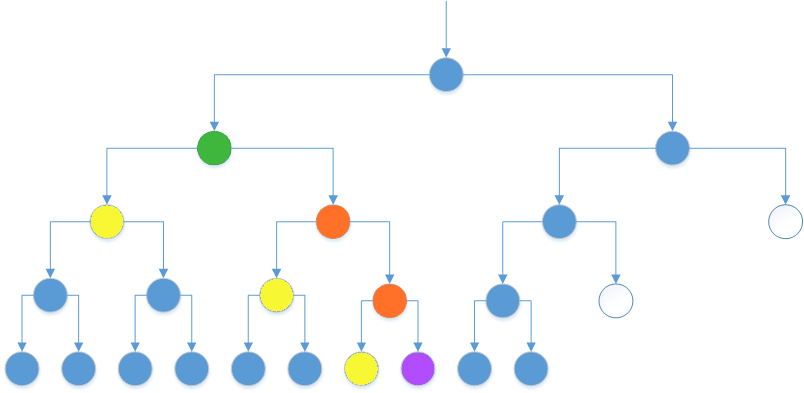
\includegraphics[width=1\textwidth]{content/pictures/TreeProof5}
	\caption{Beweis für Blatt 8}
	\label{fig:TreeProof5}
\end{figure}

Durch dieses Verfahren kann nun eine Validierung und Einfüge-Operationen in den Baum mit minimalen Informationen über den Baum realisiert werden und es müssen nicht alle Informationen über den kompletten Baum geladen werden. 

\section{Das "`Total Ordering"' Problem}
Das Total Ordering Problem beschreibt den Sachverhalt, dass in verteilten Systemen nicht immer klar festgestellt werden kann, in welcher exakten Reihenfolge Ereignisse eingetreten sind. Durch parallele Prozesse können Elemente zeitgleich bearbeitet werden. Erschwerend dazu kommt, dass die Kommunikation zwischen den Instanzen unzuverlässig und latenzbehaftet ist. In vielen Anwendungsfällen muss jedoch eine feste Reihenfolge bestimmt werden. Dies ist z.B. beim Erfassen von Systemübergreifenden Audit-Logs der Fall.\cite{359563}\\
Um diesem Problem zu begegnen, können verschiedene Mechanismen verwendet werden. Der trivialste Fall sind hochauflösende Zeitstempel. die Grundidee eines hochauflösenden Zeitstempels besagt, dass die Auflösing immer so hoch gewählt werden kann, dass zwischen beliebigen zwei Ereignissen eine zeitliche Differenz besteht. Die offensichtliche Problematik bei diesem Verfahren ist, dass es unabhängig von der Präzision des Zeitstempels, theoretisch immer trotzdem zu Kollisionen kommen kann. In verteilten Systemen gibt es außerdem ein grundsätzliches Problem: Alle Instanzen nutzen ihre eigenen Systemuhren. Um die Uhren zu synchronisieren kann ein entsprechendes Protokoll zwischen den Instanzen geschaffen werden. Hierbei ist die Herausforderung, dass die Kommunikation zwischen Instanzen latenzbehaftet ist. Latenzzeiten müssen bei der Synchronisation mit in Betracht gezogen werden. Dabei entstehen besonders dann Fehler, wenn die Latenz fluktuiert.\cite{315340}\\
Wenn zu einer zeitlichen Synchronisation im Cluster ein Protokoll zur Kommunikation zwischen den Instanzen erforderlich ist, kann man dieses Protokoll auch auf den vorliegenden Anwendungsfall spezialisieren. In einem solchen Protokoll einigen sich die Instanzen des Clusters auf eine gemeinsame Reihenfolge ohne eine zeitliche Komponente zu verwenden. Es gibt unterschiedliche Protokolle, die eine einheitliche Reihenfolge im Cluster garantieren können. Dabei unterscheiden sich zwei grundsätzliche Ansätze.\\
Im ersten Ansatz wird eine autoritäre Instanz bestimmt, über die alle anderen Instanzen die Reihenfolge erfragen müssen. Da diese Instanz eigenständig über die Reihenfolge entscheidet, wird die Reihenfolge nach der deren Bearbeitungsreihenfolge bestimmt. So kann im einfachsten Fall eine inkrementelle Sequenznummer vergeben werden. Dieses Verfahren hat folgende Nachteile: Da die Reihenfolge aller Events vieler Instanzen über eine einzelne Instanz vergeben wird, kann diese zum Engpass werden und damit die Geschwindigkeit des Gesamtsystems beeinträchtigen. Insbesondere bei Ausfällen hat dies drastische Auswirkungen auf das Gesamtsystem. Ein Lösungsansatz im Störungsfall einer autoritären Instanz wäre z.B. eine neue Instanz von allen aktiven Teilnehmern des Clusters zu wählen. Diese übernimmt dann temporär oder permanent die Funktion der ausgefallenen Instanz.\cite{565838}\\
Ein anderer Ansatz eines solchen Protokolls ist der Einsatz von Broadcasts und Majority-Voting. Wenn eine Instanz ein neues Element in die Sequenz einfügen will, wird diese Anfrage allen anderen Instanzen mitgeteilt. Wenn nun über die Hälfte der Instanzen dieses Element als das unmittelbar nächste in der Sequenz bestätigen, kann sichergestellt werden, dass das Cluster sich auf diese Reihenfolge einigt. Wenn aber die Hälfte des Clusters die Anfrage verneint, muss für die Transaktion der aktuelle Listenkopf aktualisiert und die Anfrage wiederholt werden. Diese Verfahren verursacht eine größere Netzlast, da mehr Kommunikation zwischen den Instanzen stattfinden muss, jedoch ist die Fehler und Ausfalltoleranz durch die dezentrale Struktur deutlich verbessert.\cite{1041682}\\

